\documentclass[../thesis.tex]{subfiles}
\begin{document}

In this section, we detail our new dataset, MCAC.
MCAC is the first dataset designed for multi-class class-agnostic counting. 
As discussed previously, prior to 2023, class-agnostic counting methods, including our own, presented in \Cref{sec__LTCA} and \citet{ltcahobley},  focused on enumerating instances in images where only a single class of object is present to count as this was the available data. 
This training leads to methods with very broad intra-class definitions, approximating a `generic object detector'.
In real-world applications, it is not necessarily the case that the only objects present are of the class to be counted.
While many prior methods have been assumed to generalise to multi-class settings, this has not been shown robustly.
A multi-class dataset would facilitate the evaluation of these methods on multi-class images as well as facilitate the training of new multi-class counting methods.



\subsection{Multi-Class Counting Problem Definition}
The goal of a multi-class class-agnostic counting method is to take a single image that contains multiple instances of multiple classes and return the associated counts of each.
We recognise that `\textit{exemplar-free} multi-class class-agnostic counting' is not a clearly defined task and could be interpreted as multiple different problems, each fitting a different set of requirements.
A user may only want to gain a better understanding of the distribution of objects in an image. 
However, it is likely that they would want to know a more directed piece of information, `How many objects are there of each of a set of classes that I care about?'. 
While in some contexts, it would make sense to have the user specify this preference in the form of an exemplar image or a textual description, there are cases where this would be laborious and time-consuming.
As such, we create a dataset which facilitates the training of methods to address either of the above set of requirements. We also provide extra information potentially useful for approaches we have not considered.


While the deployment query scenario, `Count given an unlabelled image of objects', is natural, the training and quantitative evaluation of methods to address it is not.
To facilitate training and evaluation of methods in multi-class settings, we need images with multiple objects of multiple types. 
To evaluate a method's generalisability to unseen object types, the classes present in the images need to be mutually exclusive between training, validation, and testing.
It is infeasible to gather natural images with (a) a wide variety of classes, (b) a wide variety of the number of times an object appears in an image, and (c) no repetition of the types of object between the train, test, and validation splits. 

While it may seem that datasets created for detection and segmentation tasks could be utilised, they generally focus on small sets of classes. Images from these datasets are also not likely to be separable into sets with mutually exclusive classes. The labelling of these classes is also generally not sufficient for many of the current class-agnostic counting methods.

Another possible solution would be to tile existing single-class images, similar to the approach taken by \citet{liu2022countr}.
While not focused on multi-class counting, \citet{liu2022countr} aimed to improve their method's class-discrimination using a tiling modification. They combined up to four images from FSC-147 to create a composite image. This was used to create a system that is more likely to count only objects similar to the exemplars rather than acting as a generic `object counter'  as many previous methods were. While this modification effectively helped with their goal of greater discrimination, it is not a robust simulation of real-world multi-class images.
This is because since the classes are spatially separable, a method can address the four corners of the image independently.
As such, this solution should not be used to evaluate a method's multi-class capabilities. 






































\subsection{Multi-Class Class-Agnostic Synthetic Dataset}
We address the problems of the previous datasets and data augmentation approaches with a new Multi-Class Class-Agnostic Counting (MCAC) dataset.
In this section, we discuss the implementation of our dataset. We explain our reason for choosing a synthetic rather than a photographic dataset.
We then discuss how the dataset was generated and the ways we think it could be used most effectively for exemplar-free and exemplar-based training. 



\subsubsection{Synthetic Choice}
There are three major constraints placed on a multi-class, class-agnostic counting dataset:
\begin{enumerate}
    \item \textbf{Multi-class} - Images should contain multiple instances of multiple types of object. 
    \item \textbf{Class-agnostic} - Classes must be mutually exclusive between training, validation and inference time. 
    \item \textbf{Diverse} - Diverse classes are required to facilitate effective training and to validate a method's generalisability.
\end{enumerate}


Gathering and labelling images that match all three constraints is prohibitively difficult. 
Due to the difficulty of producing a real dataset with accurate and consistent annotations and the flaws of augmenting single-class images, we opted to utilise synthetic data generation. While a model trained on a purely synthetic dataset may have limited application to real-world problems, we believe this gives an upper bound on the ability of a method to deal with multi-count images.
We also show in \Cref{sec__ABC123__fscresults} that a counting method trained on purely simple synthetic data can generalise well to a photographic dataset.
So it is a general and valuable tool for work on automated counting.

Two significant advantages of a synthetic dataset are the level of control we have over the composition of each image as well as the accuracy and precision of the information we can gather about the images.
The number of instances, their exact locations, their pixel-wise segmentations, and their degree of occlusion are all known to a level that would not be possible with manual labelling.
This is all achieved with minimal work, making this approach cheap, and scalable.

\subsubsection{Dataset Generation}
We generate our dataset using Blender, an open-source 3D computer graphics tool. Blender includes rendering, texturing, and physical simulation capabilities, making it ideal for our application. 
Instead of trying to find a valid packing of a large number of complex, non-convex objects without collisions or errors, we use a physics simulator to `drop' the objects from a non-colliding initialisation into a box, shown in Figure \ref{fig__blenderpredropexamples}. This creates layouts of objects with random locations and orientations, that have objects in a relatively narrow height without clipping and with realistic occlusion. 
As objects in real settings often vary in size, we vary the size of objects by $\pm$50\% from a random nominal size.
We also vary the number, location, and intensity of lights present. This somewhat evenly lights the scene allowing all objects to be seen while maintaining variation of shadow. 
We use a randomly generated multi-coloured texture as the background with random noise texture varying the surface roughness of the floor. This minimises large specular highlights while also not being simple for a network to model.
\subfile{../files/confirmation_multi_dataset/figures/blender_predropexamples.tex}

The object models are drawn from ShapeNetSem \cite{savva2015semantically}, a subset of ShapeNet \cite{shapenet2015}. Each object in ShapeNetSem is labelled hierarchically by type.
They are also pre-textured, leading to diverse and realistic appearances.
We maintain the labels from ShapeNetSem.


To enable training of various current methods \cite{ranjan2021Famnet, ranjan2022exemplar, liu2022countr} and for maximum utility in the future, 
our dataset is labelled in various ways.
Each object has associated with it a bounding box, a center-of-geometry point annotation, a final image pixel-wise segmentation, and an unoccluded segmentation. 
This is significantly more annotation information than any other class-agnostic counting dataset, as discussed in \Cref{sec__fsc133}, and more than is required by any of the contemporary methods \cite{liu2022countr, ranjan2022exemplar, shi2022represent}, as discussed in \Cref{sec__MCAC__usingMCAC,,sec__ABC123}.

We render a zoomed-out version of the final image, the final instance segmentation, and unoccluded pixel-wise segmentations of each object separately.
These zoomed-out images are such that all objects are completely within the boundaries of the image. 
From this, the occlusion percentage is calculated as:

\begin{equation}
   \text{Occlusion} = 1 - \frac{A_0}{A_1}
\end{equation}
\myequations{Occlusion Percentage}
where $A_0$ is the number of pixels in the final image segmentation and $A_1$ is the number of pixels that would be seen if the object was unoccluded and was completely within the bounds of the image.
The final images are cropped versions of the zoomed-out image.
The bounding boxes are generated from the unoccluded segmentation by finding the tightest box that includes the instance and is within the bounds of the final image.
See \Cref{fig__syntheticdatasetexamplescombined} for examples from the dataset and \Cref{fig__MCAC__moredatasetexamples} for labelled examples.

\subfile{../files/confirmation_multi_dataset/figures/multi_dataset_examples_combined.tex}



\begin{figure}
    \centering
    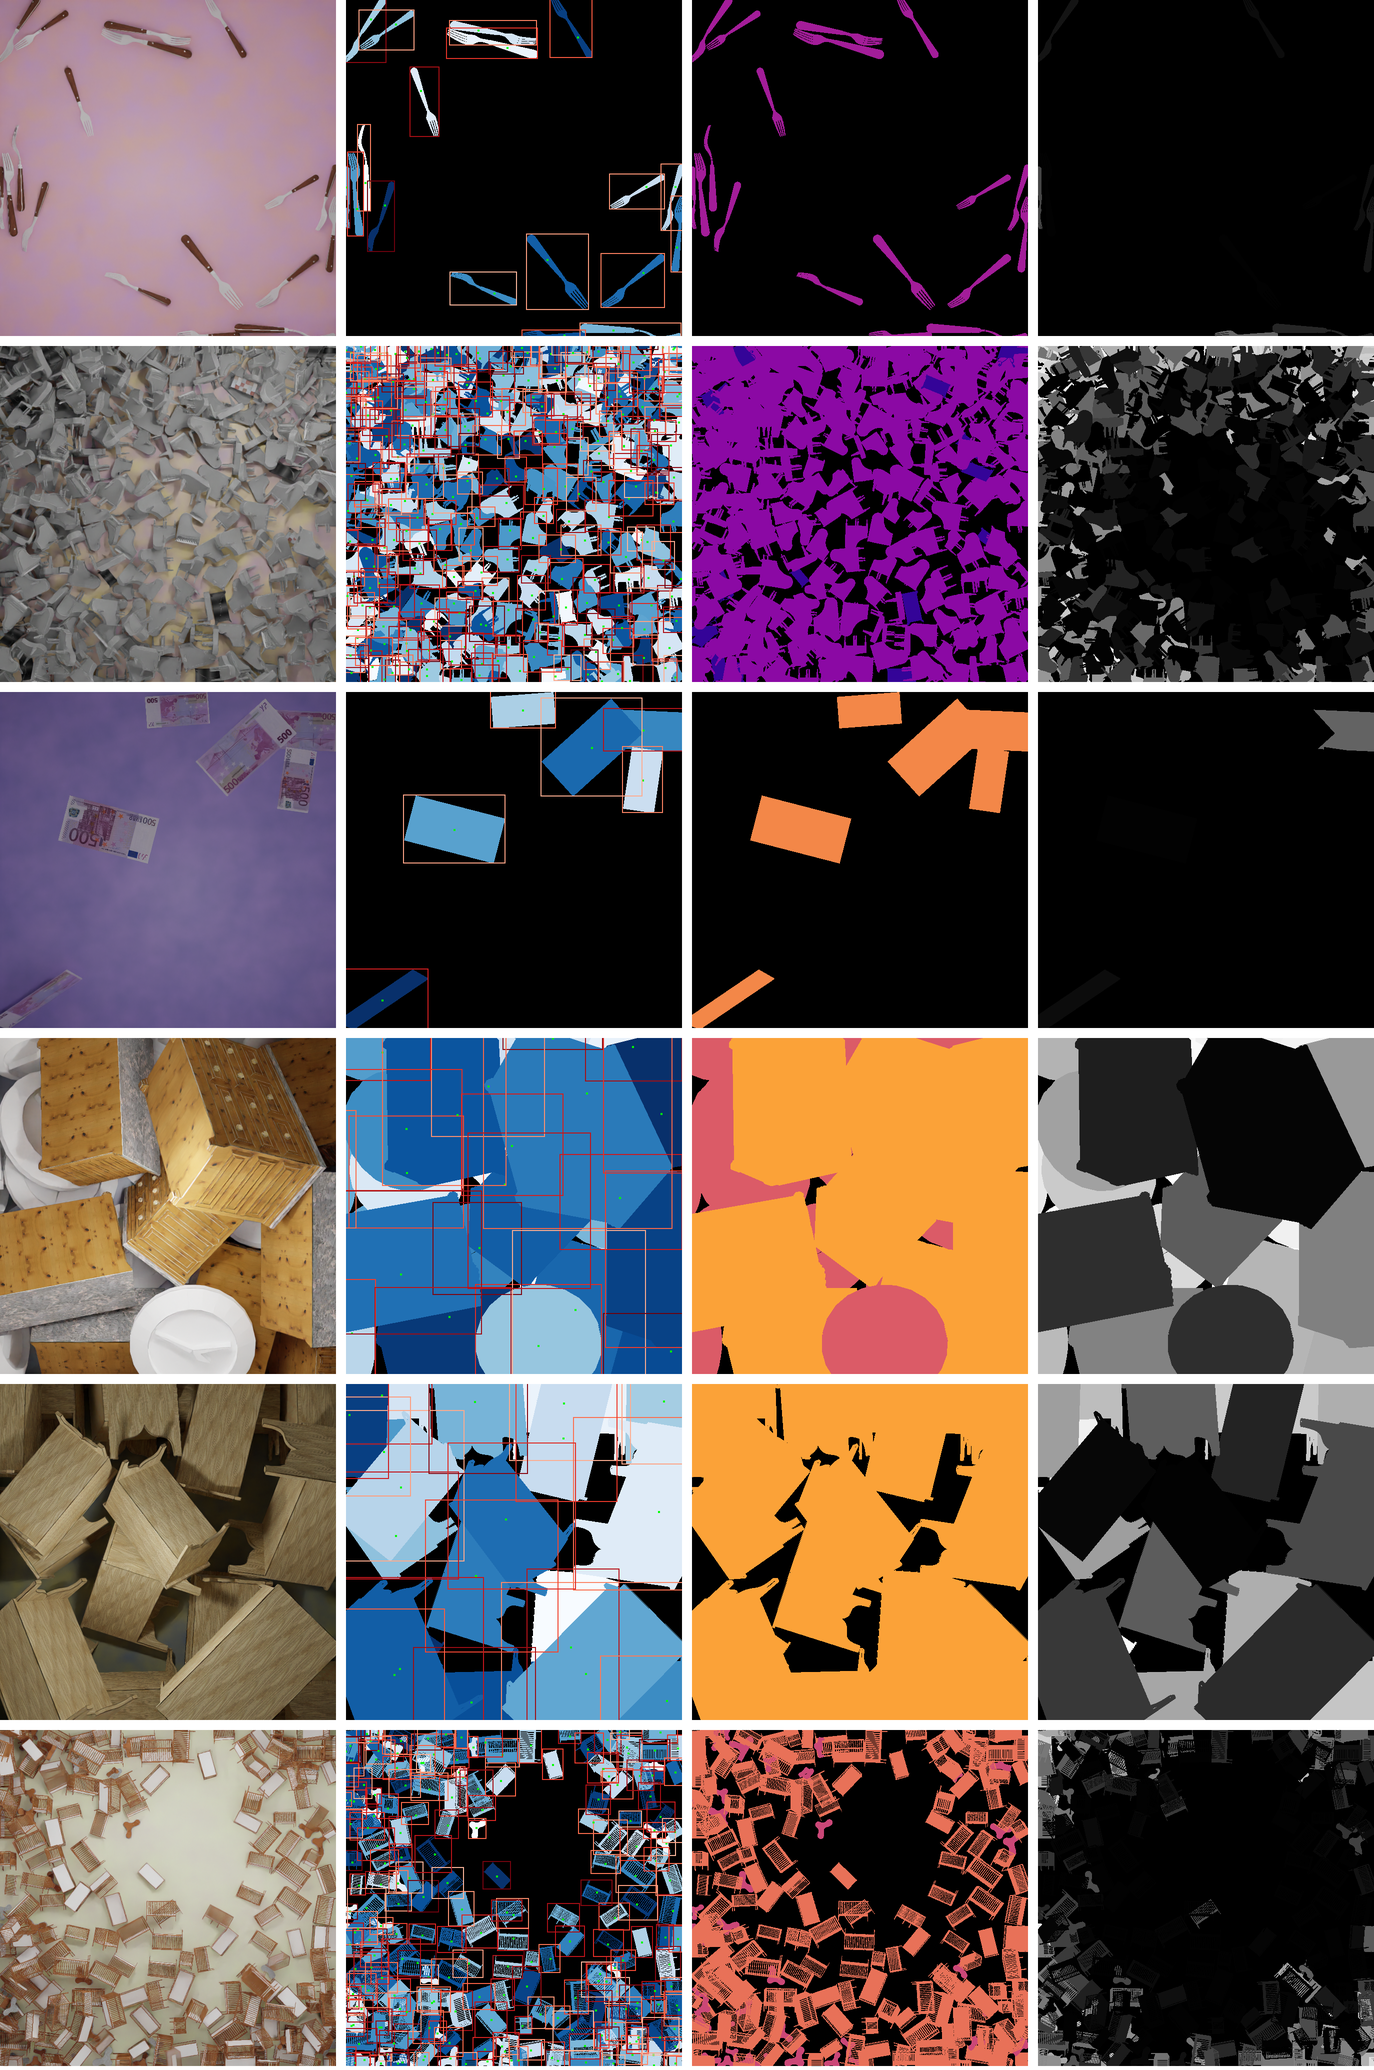
\includegraphics[width =0.9 \linewidth]{../files/confirmation_multi_dataset/images/MCAC_many_exampels(4).png}
    \caption{Labelled examples from the Multi-Class Synthetic Dataset. Each row contains a rendered image, the associated instance labels with bounding boxes and centre points, the class labels, and the individual instance occlusions.}
    \label{fig__MCAC__moredatasetexamples}
\end{figure}




\subsubsection{Dataset Breakdown}
MCAC contains images with between 1 and 4 classes of object and between 1 and 400 instances per class. The distribution of classes per image and instances per class are shown in \Cref{fig__multi_class_stats_graphs} and \Cref{tab__multiclass_dataset_stats}. 
MCAC has three data splits. The training split has 4756 images (8298 counts) drawn from 287 classes, the validation split has 2114 images (4286 counts)  drawn from 37 classes, and the testing split has 2413 images (3640 counts) drawn from 19 classes.

Many current methods were developed using images which only contain one kind of object, and so are specifically suited to this setting.
In light of this, we encourage comparisons to be made not only using MCAC but also MCAC-M1. 
MCAC-M1 is the subset of MCAC images that contain only a single class, the breakdown of which is also shown in \Cref{tab__multiclass_dataset_stats}.
Of course, the problems posed by MCAC-M1 are simpler than those posed in MCAC, where the number of classes is unknown. 
As is further discussed in \Cref{sec__ABC123__results},
we believe the discrepancy in the performance of a given method trained on MCAC and MCAC-M1 demonstrates the ability of the method to discriminate between objects based on type rather than acting as a generic object counter. 

\subfile{../files/confirmation_multi_dataset/tables/multiclass_dataset_stats.tex}
\subfile{../files/confirmation_multi_dataset/figures/multi_class_stats_graphs.tex}
\subsubsection{Ambiguity}
Both exemplar-based and exemplar-free methods bump into problems of ambiguity. If there are objects of varied levels of generality, which boundary should be used? 
For example, on a chess board with a single white pawn as the exemplar, should the count be of all the pieces, all the white pieces, all the white pawns, all the pawns, and so on? 

Given the infeasibility of defining every possible way of grouping the objects present in an image, we define a single way of grouping them: an identical mesh and texture, independent of size or orientation. 
We do, however, acknowledge the existence of other 
\textit{valid-but-unknown} counts, the unlabelled ways of grouping the objects, introduced in \Cref{sec__lit_rev__count_valid_but_unkonwon_counts}. 
As the original class hierarchy labels are preserved, future works could count based on more complex definitions of similarity than we utilise.

\subsubsection{Dataset Usage}\label{sec__MCAC__usingMCAC}
Here, we outline a set of standards we suggest for the dataset when it is used in future works and that we follow in our later work. These are by no means the only way the dataset can be used, and the segmentations, hierarchical class labels, and occlusion labels allow for much more complex and interesting use cases.


We group objects as the same if they share the same geometry and texture, independent of their orientation or size.
As was asserted by \citet{ranjan2021Famnet}, an object that can barely be seen or recognised should not be counted. While it is difficult to define these terms robustly for photographic data, our use of synthetic data allows us to set a consistent, quantitative boundary. We exclude from the final count all objects that are more than 70\% occluded by either other objects or the edge of the frame. 
Though true density maps could be utilised as we have instance-wise segmentations,  we use ground-truth pseudo-density maps to align with prior methods' approaches \cite{ranjan2021Famnet, liu2022countr, yang2021cfoc, lin2021object}. These pseudo-density maps have a Gaussian kernel centred on the centre of geometry of each object with $\sigma = 8$.
As is standard, when the Gaussians from different instances overlap, we sum them rather than taking the maximum value. 
As some of the Gaussian kernels are cut off by the edge of the frame, the sum of the density maps will be lower than the desired integer count labels.
We scale each density map so the sum over it is the correct value. This adjustment to the training data improved our results on the test data by $\sim5\%$.

To ensure that meaningful but varied exemplars are used during the training of exemplar-based methods, we take bounding boxes randomly from instances with less than 30\% occlusion.
We evaluate these methods using the bounding boxes of the three least occluded instances. In cases with more than three equally occluded instances, we use those with the lowest instance IDs. 

\subsection{Conclusion}
In this chapter, we have proposed two datasets, FSC-133 and MCAC.
FCS-133 improves upon the current most popular class-agnostic counting dataset, FSC-147, by removing errors and ambiguities. 
We believe these improvements not only facilitate more representative evaluation but also lead to methods being able to learn a more consistent understanding of counting. 
MCAC addresses what we see as the most significant limitation of current class-agnostic counting datasets, that they are single-class.
MCAC is the first multi-class class-agnostic counting dataset. 
It features diverse object types and counts and is labelled with a high level of accuracy and consistency.
As seen in \Cref{sec__ABC123}, MCAC enables the training of exemplar-based and exemplar-free multi-class counting methods. 
It also allowed us to show that methods previously believed to generalise from single-class training into multi-class settings do not in fact achieve this.
Both datasets provide significant utility to our work as well as the broader field of class-agnostic counting as a whole.

\end{document}
